\chapter{Experimental and processing approaches}
\label{chap:experimental-processing-approaches}

This chapter defines the experimental and methodological framework used to evaluate the feasibility of optical tether observation and geometric reconstruction under representative orbital-like conditions. Based on the optical and radiometric constraints established previously, the methodology was designed to progressively evaluate the limitations of conventional reconstruction methods and validate alternative approaches specifically adapted to thin, textureless tether structures.
\\\\
The proposed validation strategy follows a progressive transition from conventional feature-based photogrammetry toward geometry-driven reconstruction and exploratory AI-assisted processing. Rather than treating all reconstruction approaches equivalently, the methodology intentionally prioritizes physically interpretable geometric extraction methods capable of operating under sparse visual conditions and extreme radiometric contrast.
\\\\
The complete framework is organized into three global development phases:

\begin{itemize}
    \item Phase I: Evaluation of conventional photogrammetry methods under terrestrial and space-emulated visual conditions to establish the operational limitations of standard feature-matching approaches.
    \item Phase II: Development and validation of a custom geometry-driven reconstruction pipeline based on edge extraction, radiometric centroiding, and stereo geometric constraints.
    \item Phase III: Exploratory evaluation of AI-assisted reconstruction techniques intended to support future improvements in segmentation robustness and complex topology reconstruction.
\end{itemize}

Together, these phases establish a progressive methodological roadmap for the LINKU stereo vision system.
\newpage
\clearpage

\begin{figure}[!ht]
    \centering
    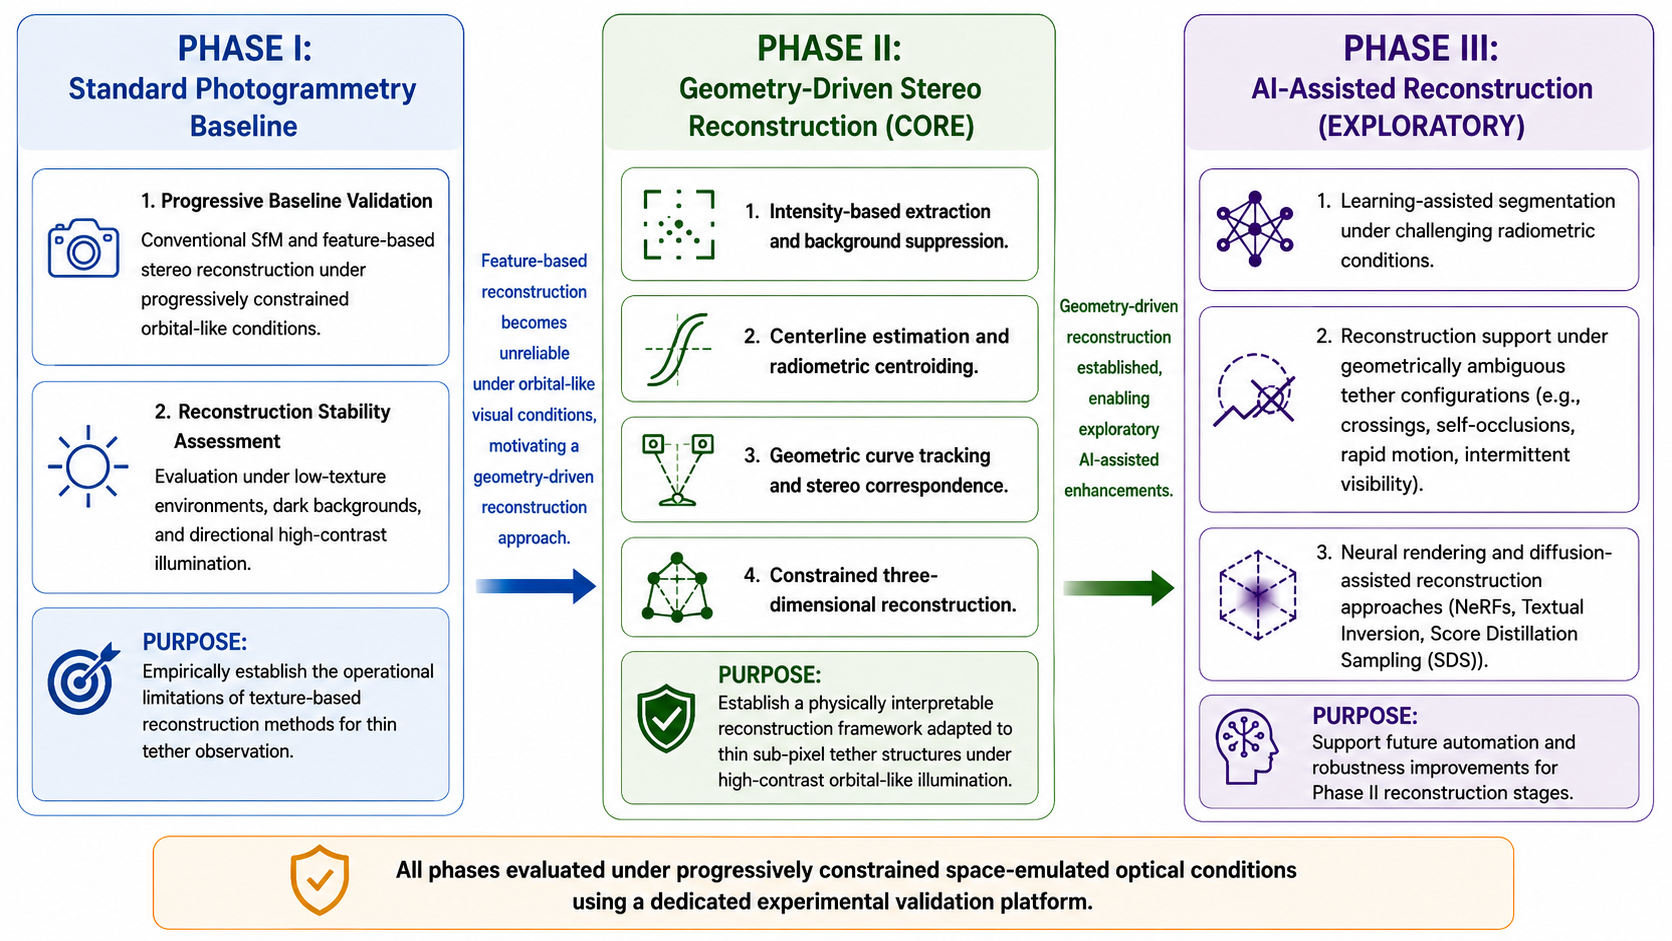
\includegraphics[width=\textwidth]{Images/Figure 4.1.png}
    \caption[Methodological roadmap of the LINKU stereo vision system validation strategy]{Methodological roadmap of the LINKU stereo vision system validation strategy. The framework progressively transitions from conventional texture-based photogrammetry toward a geometry-driven stereo reconstruction methodology and exploratory AI-assisted enhancements under increasingly constrained orbital-like optical conditions. The roadmap highlights the progressive evolution from feature-based reconstruction failure analysis to physically interpretable tether reconstruction adapted to thin sub-pixel structures.}
    \label{fig:figure4.1}
\end{figure}

Rather than directly attempting end-to-end reconstruction under fully space-emulated conditions, the proposed methodology progressively isolates the principal failure modes associated with thin tether observation, including low texture, sub-pixel geometry, directional illumination, and radiometric instability.
\\\\
This progressive validation strategy enables analysis of the reconstruction problem with increasing optical and computational complexity while maintaining traceability between the optical constraints identified in Chapter 3 and the observed reconstruction behavior under representative orbital-like conditions.
\\\\
As a result, the framework establishes a transition from conventional texture-based photogrammetry to a dedicated geometry-driven stereo reconstruction methodology adapted to thin, sub-pixel tether structures under high-contrast, orbital-like illumination.

\section{Phase I: Standard photogrammetry baseline}

Phase I establishes the experimental baseline used to evaluate conventional photogrammetry methods under progressively constrained visual conditions representative of orbital tether observation. Its purpose is to empirically establish the operational limitations of conventional texture-based photogrammetry for thin tether observation under representative orbital-like optical conditions.
\\\\
This phase assesses the applicability of feature-based stereo reconstruction approaches to geometries and illumination conditions relevant to the LINKU mission. In particular, the methodology evaluates the influence of:

\begin{itemize}
    \item Environmental texture
    \item Geometric scale
    \item Directional illumination
    \item High-contrast backgrounds
\end{itemize}

On the operation of conventional Structure-from-Motion (SfM) and stereo matching algorithms.
\\\\
The experiments were conducted using Agisoft Metashape as the reference photogrammetry platform. The evaluation considered:

\begin{itemize}
    \item Camera alignment behavior
    \item Disparity-map generation
    \item Stereo correspondence consistency
    \item Point-cloud reconstruction capability
\end{itemize}

As illustrated in the methodological roadmap presented in Figure 4.1, the Phase I methodology is organized into two principal processing stages:

\vspace{0.5cm}
\noindent \textbf{Progressive baseline validation}
\vspace{0.2cm}

Phase I was structured as a progressive validation sequence intended to incrementally approximate the optical conditions expected during orbital tether observation.
\\\\
The methodology begins with the reconstruction of a volumetric object containing easily distinguishable geometric features under controlled environmental conditions. This initial stage establishes a reference baseline for evaluating conventional feature-based reconstruction behavior under textured terrestrial environments.
\\\\
Subsequently, the validation sequence transitions toward thin tether observation using a tether proxy operating under progressively constrained visual conditions. This progression allows evaluation of conventional stereo reconstruction methods as the observed geometry evolves from feature-rich volumetric structures toward thin sub-pixel line-like objects representative of the LINKU operational scenario.

\vspace{0.5cm}
\noindent \textbf{Reconstruction stability assessment}
\vspace{0.2cm}

This second stage evaluates reconstruction stability under progressively constrained visual environments representative of orbital-like observation conditions.
\\\\
The analysis considers the influence of:

\begin{itemize}
    \item Reduced environmental texture
    \item Dark backgrounds
    \item Directional high-contrast illumination
    \item Geometric scale reduction
\end{itemize}

On the stability of conventional photogrammetry algorithms.
\\\\
Particular attention is placed on evaluating:

\begin{itemize}
    \item Camera alignment stability
    \item Disparity-map consistency
    \item Stereo correspondence reliability
    \item Point-cloud reconstruction capability
\end{itemize}

Under conditions where conventional texture-based feature matching becomes increasingly limited.
\\\\
This validation framework establishes a controlled methodological progression for evaluating the operational applicability of conventional photogrammetry, as shown in Figure \ref{fig:figure4.2}, prior to implementing the geometry-driven reconstruction methodology introduced in Phase II.

\begin{figure}[!ht]
    \centering
    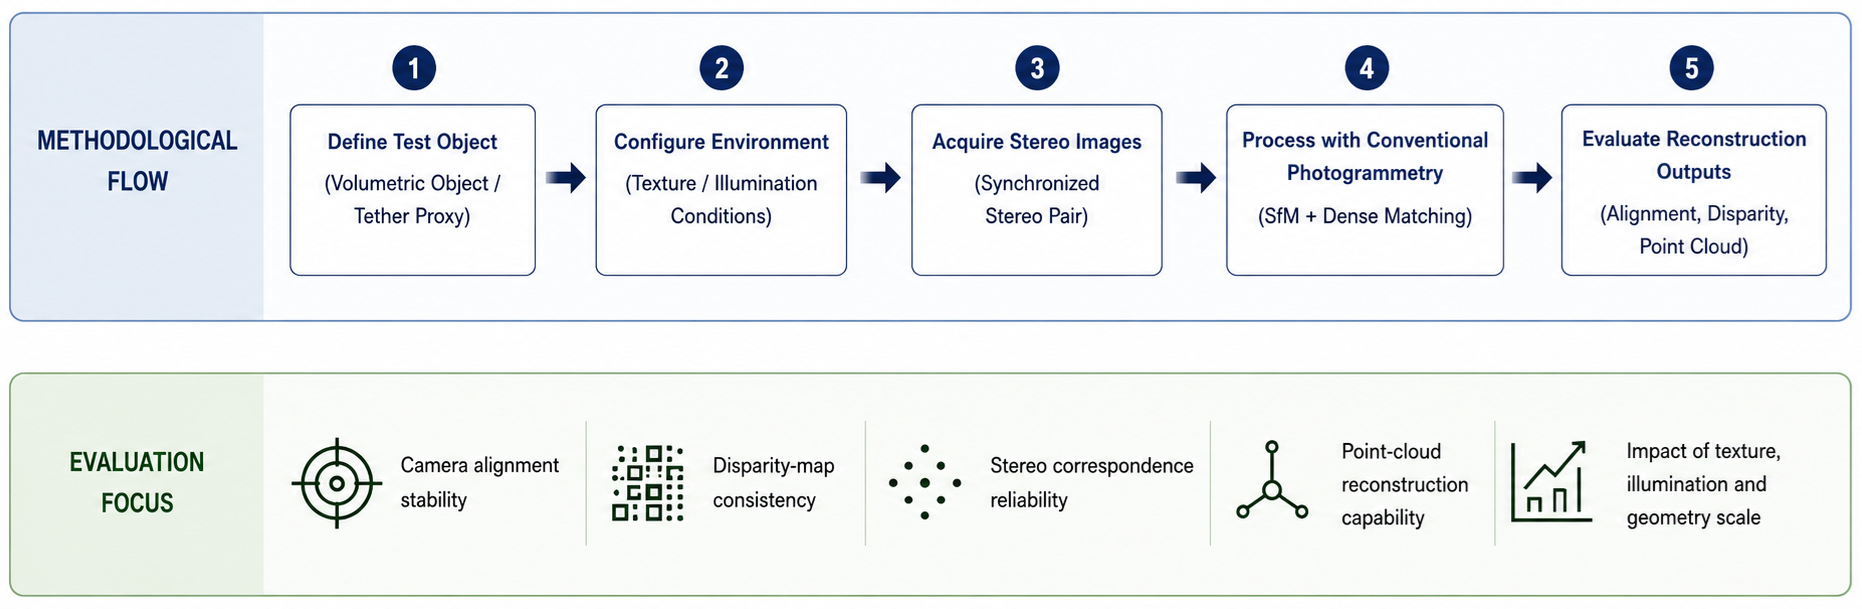
\includegraphics[width=\textwidth]{Images/Figure 4.2.png}
    \caption[Methodological flow and evaluation focus adopted during Phase I]{Methodological flow and evaluation focus adopted during Phase I. The validation sequence progressively transitions from controlled volumetric-object reconstruction toward thin tether observation under increasingly constrained orbital-like optical conditions.}
    \label{fig:figure4.2}
\end{figure}

\vspace{0.5cm}
\noindent \textbf{Traditional dense stereo pathway retained in the current software}
\vspace{0.2cm}

Alongside the external Agisoft Metashape experiments described above, the LINKU software itself still retains a conventional, cable-agnostic dense stereo processing path. It is not a separate tool: it is the same \texttt{process\_stereo\_pair} routine used throughout this work, running with no cable mask supplied, which is exactly what happens if the operator skips the segmentation-tuning step described in Phase II. Figure \ref{fig:pipeline-phase1-dense-stereo} shows this pathway for completeness, since it remains available in the current implementation as the software's own conventional/baseline processing mode, distinct from the dedicated geometry-driven pipeline introduced in Phase II.

\begin{figure}[!ht]
    \centering
    \resizebox{\textwidth}{!}{%
    \begin{tikzpicture}[
        font=\scriptsize,
        node distance = 9mm,
        stage/.style   = {rectangle, draw, rounded corners, fill=gray!8,
                          text width=2.7cm, align=center, minimum height=1.5cm},
        note/.style    = {text width=2.7cm, align=center, font=\tiny, text=black!65},
        arr/.style     = {-{Stealth[length=2mm]}, thick},
    ]

    \node[stage] (capture)   {\textbf{1. Capture}\\Synchronized stereo pair};
    \node[stage, right=of capture] (rect)  {\textbf{2. Rectification}\\Calibration $\rightarrow$ aligned epipolar rows};
    \node[stage, right=of rect]    (disp)  {\textbf{3. Dense disparity}\\SGBM or BM block matching, whole image};
    \node[stage, right=of disp]    (filt)  {\textbf{4. Filtering}\\WLS + bilateral smoothing};
    \node[stage, right=of filt]    (conf)  {\textbf{5. Confidence mask}\\Automatic, rejects isolated/noisy pixels};
    \node[stage, right=of conf]    (cloud) {\textbf{6. Depth \& point cloud}\\Triangulation via calibration matrix};

    \draw[arr] (capture) -- (rect);
    \draw[arr] (rect) -- (disp);
    \draw[arr] (disp) -- (filt);
    \draw[arr] (filt) -- (conf);
    \draw[arr] (conf) -- (cloud);

    \node[note, below=4mm of conf] {No cable-specific segmentation involved -- the whole image is matched};

    \end{tikzpicture}}
    \caption[Traditional dense stereo pipeline still present in the current software]{Traditional dense stereo pipeline still present in the current software (\texttt{processing/stereo\_processor.py}, \texttt{process\_stereo\_pair}). This is the pathway the software falls back to automatically whenever no cable-specific mask has been configured through the segmentation tuner: it treats the whole image as a conventional dense stereo scene, with no thread-specific extraction step. The confidence mask (stage 5) is generated automatically from local disparity consistency and pixel density, not from a manually or AI-selected filter, and is used to discard unreliable points before triangulation. This pathway corresponds to the dense-stereo experiment discussed in Section \ref{sub:volumetric-object-reconstruction}, where the absence of a cable-specific mask allowed background disparity artifacts to propagate into the reconstruction.}
    \label{fig:pipeline-phase1-dense-stereo}
\end{figure}


\section{Phase II: Geometry-driven stereo reconstruction}
\label{sec:Geometry-driven stereo reconstruction}

Phase II is the primary reconstruction approach of the LINKU camera system. After explaining the methodological limitations identified during Phase I, Phase II introduces a dedicated reconstruction framework tailored to thin tether structures operating under low-texture, high-contrast, orbital-like optical conditions.
\\\\
Unlike conventional photogrammetry approaches, the proposed methodology does not rely primarily on texture-based feature correspondence. Instead, the reconstruction strategy treats the tether as a continuous geometric structure whose detectability is governed mainly by radiometric contrast, geometric continuity, and constrained stereo geometry, as shown in Figure \ref{fig:figure4.3}.
\\\\
This phase establishes a physically interpretable reconstruction methodology that operates under the sub-pixel observation conditions derived in Chapter 3.
\newpage
\clearpage

\begin{figure}[!ht]
    \centering
    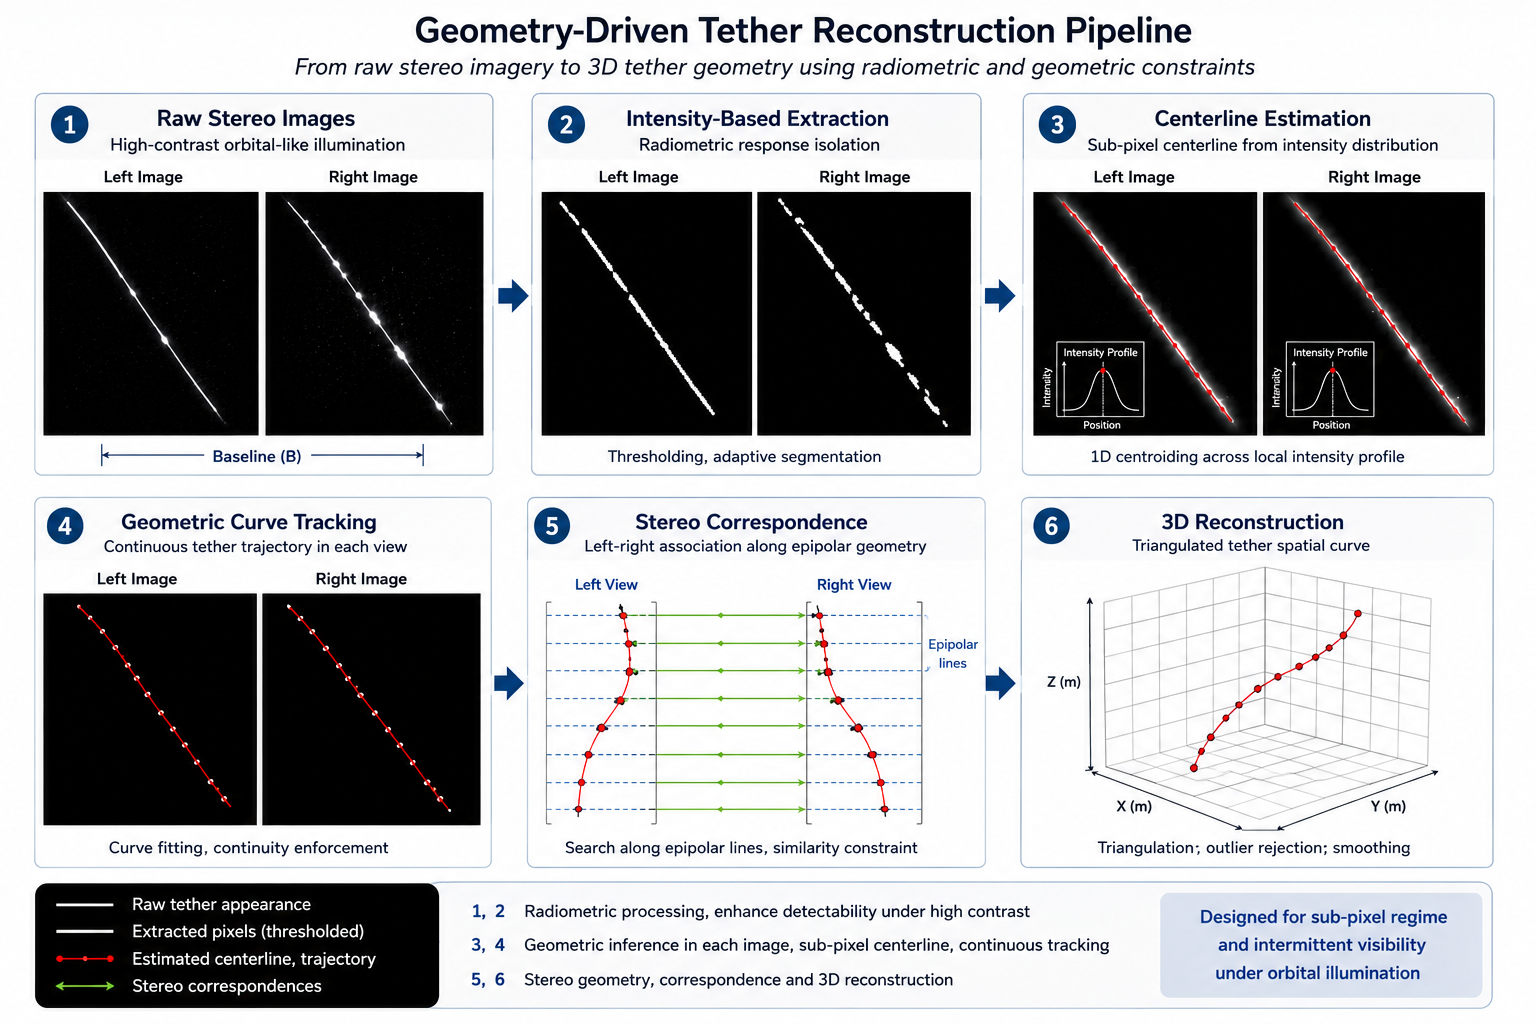
\includegraphics[width=\textwidth]{Images/Figure 4.3.png}
    \caption[Conceptual overview of the geometry-driven reconstruction pipeline proposed for thin tether observation in the sub-pixel regime]{Conceptual overview of the geometry-driven reconstruction pipeline proposed for thin tether observation in the sub-pixel regime. The workflow illustrates the progressive transition from raw stereo image acquisition under high-contrast orbital-like illumination toward constrained three-dimensional tether reconstruction. The methodology includes: (1) acquisition of synchronized stereo images, (2) intensity-based tether extraction and background suppression, (3) sub-pixel centerline estimation through radiometric centroiding, (4) geometric curve tracking for continuous tether representation, (5) stereo correspondence establishment using epipolar geometric constraints, and (6) three-dimensional reconstruction through triangulation of the stereo-associated tether geometry. The figure highlights the transition from conventional texture-dependent processing toward radiometric and geometry-driven reconstruction methods adapted to thin low-texture structures under orbital-like optical conditions.}
    \label{fig:figure4.3}
\end{figure}

Figure \ref{fig:figure4.3} presents the conceptual view of this pipeline. Figure \ref{fig:pipeline-implementation} complements it by naming the specific algorithms used in the current software implementation, including the classical and AI-assisted variants evaluated for each stage.

\begin{figure}[!ht]
    \centering
    \resizebox{\textwidth}{!}{%
    \begin{tikzpicture}[
        font=\scriptsize,
        node distance = 9mm,
        stage/.style   = {rectangle, draw, rounded corners, fill=blue!8,
                          text width=2.7cm, align=center, minimum height=1.5cm},
        note/.style    = {text width=2.7cm, align=center, font=\tiny, text=black!65},
        arr/.style     = {-{Stealth[length=2mm]}, thick},
    ]

    \node[stage] (capture)  {\textbf{1. Capture}\\Synchronized stereo pair};
    \node[stage, right=of capture]  (seg)      {\textbf{2. Segmentation}\\Image $\rightarrow$ binary cable mask};
    \node[stage, right=of seg]      (endpoints){\textbf{3. Endpoints}\\Mask $\rightarrow$ the two loose ends};
    \node[stage, right=of endpoints](track)    {\textbf{4. Path tracing}\\Ends $\rightarrow$ ordered points along the thread};
    \node[stage, right=of track]    (match)    {\textbf{5. Stereo matching}\\Left/right path correspondence};
    \node[stage, right=of match]    (metrics)  {\textbf{6. Triangulation}\\3D coordinates \& metrics};

    \draw[arr] (capture) -- (seg);
    \draw[arr] (seg) -- (endpoints);
    \draw[arr] (endpoints) -- (track);
    \draw[arr] (track) -- (match);
    \draw[arr] (match) -- (metrics);

    \node[note, below=4mm of seg]   {HSV threshold (classical) \emph{or} Random Forest classifier (AI, implemented)};
    \node[note, below=4mm of track] {SmartWireTracker search (classical, implemented) \emph{or} learned scorer (AI, proposed)};

    \end{tikzpicture}}
    \caption[Implementation-level view of the Phase II reconstruction pipeline]{Implementation-level view of the Phase II (geometry-driven) reconstruction pipeline. The six boxes are the processing stages, each labeled with the transformation it performs. Where a stage currently offers more than one implementation -- segmentation and path tracing -- the classical method already implemented and the AI-assisted alternative are noted underneath; all other stages have a single, classical implementation today. Algorithm-level detail for each stage is given in the surrounding text rather than in the diagram.}
    \label{fig:pipeline-implementation}
\end{figure}


As illustrated in the methodological roadmap presented in Figure 4.1, the Phase II methodology is organized into four principal processing stages:

\vspace{0.5cm}
\noindent \textbf{Intensity-based extraction and background suppression}
\vspace{0.2cm}

Once stereo images have been acquired from both cameras, the reconstruction process begins with intensity-based extraction and background suppression under controlled illumination conditions designed to maximize radiometric contrast between the tether and the surrounding background. Since the orbital environment is expected to exhibit minimal texture, the methodology prioritizes isolating radiometric response and localized contrast enhancement over conventional feature extraction.
\\\\
This initial stage focuses on isolating the tether's radiometric signature while minimizing the effects of background noise, localized reflections, and non-uniform illumination.
\\\\
Under sub-pixel observation regimes, the tether may no longer remain conventionally observable as a fully resolvable geometric structure. Instead, its detectability becomes increasingly dependent on the isolation of localized intensity variations generated within the image plane.
\\\\
The resulting segmented representation establishes the initial geometric reference used for the subsequent centerline estimation and stereo reconstruction stages.

\noindent \textbf{Centerline estimation and radiometric centroiding}
\vspace{0.2cm}

Following intensity-based extraction and background suppression, the tether is represented in both stereo images as a thin line-like radiometric structure whose apparent position must be estimated with sub-pixel precision.
\\\\
At this stage, the methodology estimates the geometric centerline of the tether and its radiometric centroid from localized intensity distributions. Instead of relying on conventional textured keypoints, the reconstruction framework uses edge-based localization and radiometric analysis to estimate the apparent tether trajectory in the image plane.
\\\\
This approach is conceptually aligned with line-profile analysis methods such as Steger's framework \cite{steger2000subpixel}, in which line-like structures are characterized by local intensity gradients and scale-space behavior. In this context, centerline estimation allows the tether to be represented as a continuous geometric trajectory inferred from its radiometric response rather than from explicitly resolvable geometric boundaries.
\\\\
Under sub-pixel observation conditions, radiometric centroiding becomes particularly important because the tether may no longer remain fully observable as a conventionally resolvable structure. Consequently, the apparent tether position is estimated from the radiometric distribution associated with the observed line response, enabling sub-pixel localization of the tether trajectory prior to stereo correspondence and three-dimensional reconstruction.

\vspace{0.5cm}
\noindent \textbf{Geometric curve tracking and stereo correspondence}
\vspace{0.2cm}

Once the tether centerline has been estimated in both stereo views, the methodology performs geometric curve tracking and stereo correspondence in order to establish consistent associations between the tether trajectories observed in each image plane.
\\\\
Rather than treating the tether as a collection of independent feature points, the reconstruction framework models it as a continuous geometric structure whose trajectory can be constrained spatially and radiometrically across both stereo observations. This approach prioritizes geometric continuity and trajectory coherence instead of conventional dense texture matching.
\\\\
At this stage, epipolar geometry is used to constrain the stereo correspondence search along the extracted tether trajectories, reducing ambiguity in low-texture regions and improving geometric consistency between both image planes.
\\\\
Because the tether behaves as a continuous line-like structure under sub-pixel observation conditions, geometric curve tracking becomes particularly important for preserving trajectory continuity during stereo association. Consequently, the methodology prioritizes constrained stereo correspondence and continuous geometric tracking rather than independent point-feature matching.

\vspace{0.5cm}
\noindent \textbf{Constrained three-dimensional reconstruction}
\vspace{0.2cm}

The final stage of the methodology consists of constrained three-dimensional reconstruction based on the stereo correspondence relationships established between both image planes.
\\\\
At this stage, the stereo-associated tether trajectories are processed using constrained stereo geometry to infer the three-dimensional spatial configuration of the tether under sub-pixel observation conditions. Unlike conventional dense photogrammetry approaches, the methodology does not seek to reconstruct volumetric point clouds or texture-rich surfaces. Instead, the reconstruction framework focuses on recovering the continuous geometric behavior of the tether throughout the observed operational range.
\\\\
The primary objective of this stage is to reconstruct the spatial trajectory of the tether, curvature evolution, oscillatory behavior, and temporal geometric dynamics.

Because the tether behaves as a continuous, line-like structure with limited geometric observability, the reconstruction process prioritizes trajectory continuity and constrained geometric consistency across stereo observations over dense feature correspondence.
\\\\
The resulting framework establishes the primary operational reconstruction methodology of the LINKU stereo vision system and serves as the basis for the experimental hardware implementation and validation environments described in Chapter 5.

\section{Phase III: AI-Assisted reconstruction (Exploratory)}
 
Phase III investigates the future integration of Artificial Intelligence (AI) techniques intended to complement the geometry-driven reconstruction framework established in Phase II.
\\\\
This phase will not replace the deterministic reconstruction methodology based on constrained stereo geometry, geometric curve tracking, and radiometric localization, but rather evaluate the potential of AI-assisted approaches to improve the robustness of intensity-based extraction, geometric trajectory continuity, and operation under visually ambiguous conditions.
\\\\
As illustrated in the methodological roadmap in Figure \ref{fig:figure4.1}, the exploratory AI-assisted framework primarily supports the reconstruction stages already established during Phase II.
\newpage
\clearpage

\noindent \textbf{Current implementation status}
\vspace{0.2cm}

Phase III groups together three AI-related directions with markedly different levels of maturity. Rather than presenting all three as equally exploratory, this report distinguishes explicitly between the direction that has already produced a working implementation, the direction for which only data-collection infrastructure exists, and the direction that remains a documented idea without any corresponding code. Figure \ref{fig:ai-status} summarizes this distinction, which is elaborated in the three subsections below.

\begin{figure}[!ht]
    \centering
    \resizebox{\textwidth}{!}{%
    \begin{tikzpicture}[
        font=\small,
        row/.style   = {rectangle, draw, rounded corners, minimum height=1.5cm,
                        text width=4.6cm, align=left, inner sep=3mm},
        tag/.style   = {rectangle, draw, rounded corners, minimum height=1.5cm,
                        text width=8.4cm, align=left, font=\scriptsize, inner sep=3mm},
        implemented/.style = {row, draw=green!45!black, fill=green!10},
        tagimpl/.style     = {tag, draw=green!45!black, fill=green!5},
        partial/.style     = {row, draw=orange!70!black, fill=orange!10, dashed},
        tagpartial/.style  = {tag, draw=orange!70!black, fill=orange!5, dashed},
        node distance = 6mm and 6mm,
    ]

    \node[implemented] (m1) {\textbf{1. Cable segmentation}\\Random Forest, pixel-level};
    \node[tagimpl, right=of m1] (t1) {\textbf{Implemented \& trained.} 9 features (BGR+HSV+local contrast), 6 stereo pairs $\rightarrow$ 60 augmented images, F1 = 0.97 (train set, no held-out validation yet). Integrated as a selectable inference mode in the segmentation tuner.};

    \node[partial] (m2) [below=of m1] {\textbf{2. AI wire path tracker}\\(covers both ordinary tracking \emph{and} knot / crossing resolution -- one model, one purpose: given a thread image, tangled or not, trace its path without errors)};
    \node[tagpartial, right=of m2] (t2) {\textbf{Dataset collection only.} Stereo pairs with drawn/tracker-verified paths are stored (1 sample so far, $\geq$30--100 recommended). No model has been trained. Section \ref{sec:Geometry-driven stereo reconstruction} (Figure \ref{fig:ai-proposed-tracker}) proposes a concrete architecture: a learned per-branch scorer inserted into the existing search, so the same model resolves both untangled and knotted configurations.};

    \end{tikzpicture}}
    \caption[Current maturity of the two AI-related components in the LINKU camera system software]{Current maturity of the two AI-related components considered within the LINKU camera system software, as of the software state accompanying this report. Only the segmentation model (1) is operational today. Wire path tracking and topological knot/crossing resolution (2) are treated as a single AI component -- not two separate systems -- because both solve the same underlying problem: given a segmented thread image, determine the correct continuous path from one end to the other, regardless of how entangled the thread is.}
    \label{fig:ai-status}
\end{figure}


\noindent \textbf{1. Learning-assisted intensity-based extraction}
\vspace{0.2cm}

The first exploratory direction considers using learning-based methods to improve intensity-based extraction and background suppression under challenging radiometric conditions.
\\\\
Although the deterministic extraction approach developed in Phase II prioritizes physically interpretable processing, AI-assisted methods may provide additional robustness under conditions involving non-uniform illumination, intermittent tether visibility, partial saturation, and localized blooming artifacts, as shown in Figure \ref{fig:figure4.4}.
\\\\
Unlike the other two exploratory directions discussed in this section, this direction has already produced a first working implementation, integrated into the same laboratory software used for the Phase II experiments. A pixel-level Random Forest classifier was trained to segment the tether from the background, using nine features per pixel (RGB, HSV, and a local-contrast measure derived from a difference of Gaussian blurs). The training set consisted of 6 manually annotated stereo pairs, expanded to 60 images through horizontal/vertical flipping and brightness augmentation ($\pm$35 levels), and evaluated with an F1-score of 0.97 (precision 0.94, recall 0.99). This evaluation was performed on the training set itself; a held-out validation split has not yet been implemented, so the reported score should be read as an upper bound on current performance rather than a generalization estimate. The trained model is selectable as an alternative to manual HSV thresholding directly within the segmentation tuning interface, and every new mask produced through either method can be added to the training set, allowing the model to be iteratively re-trained as more laboratory sessions are collected.
\\\\
Potential further approaches include:

\begin{itemize}
    \item Convolutional neural networks (CNNs), which would replace the current hand-crafted per-pixel features with learned spatial features
    \item Full semantic segmentation architectures (e.g. U-Net-style encoder-decoders)
    \item Hybrid image-enhancement pipelines
\end{itemize}

This stage assists the intensity-based extraction and background suppression processes while preserving compatibility with the geometry-driven reconstruction framework established in Phase II.

\begin{figure}[!ht]
    \centering
    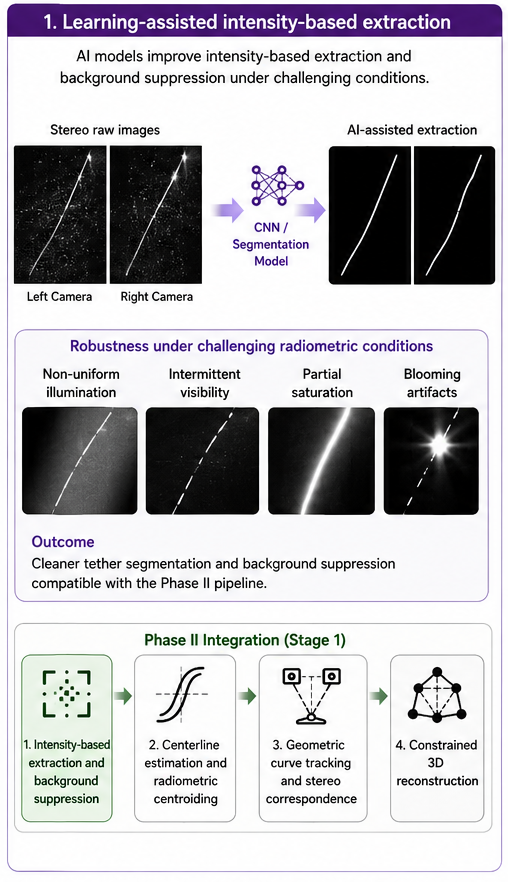
\includegraphics[width=0.5\textwidth]{Images/Figure 4.4.png}
    \caption[Conceptual overview of learning-assisted intensity-based extraction under challenging radiometric conditions]{Conceptual overview of learning-assisted intensity-based extraction under challenging radiometric conditions. AI-based segmentation approaches are investigated to improve tether extraction and background suppression in scenarios involving non-uniform illumination, intermittent visibility, partial saturation, and localized blooming artifacts. This stage enhances the robustness of the initial radiometric extraction process while preserving compatibility with the deterministic geometry-driven framework.}
    \label{fig:figure4.4}
\end{figure}
\newpage
\clearpage

\noindent \textbf{2. AI-assisted wire path tracking (including knot / crossing resolution)}
\vspace{0.2cm}

The second exploratory direction investigates the use of AI-assisted methods to support geometric curve tracking and stereo correspondence under geometrically ambiguous tether configurations.
\\\\
This includes scenarios involving tether crossings, partial self-occlusion, rapid oscillatory motion, and discontinuous radiometric visibility, as seen in Figure \ref{fig:figure4.5}. Earlier drafts of this report discussed ``learning-assisted path tracking'' and ``topological knot solving'' as two separate future capabilities. They are treated here as a single AI component instead, because they solve the same underlying problem: given a segmented thread image, determine the correct continuous path from one end to the other. An untangled thread simply presents fewer ambiguous decision points along that path than a self-crossing or knotted one.
\\\\
This direction is presently at an earlier stage than the segmentation model described above. The current software already collects the training data it would require: every path traced through the deterministic tracker, or drawn manually by an operator, is stored together with its stereo image pair and segmentation mask in a dedicated dataset (1 stereo sample so far; 30--100 are recommended before training is attempted). However, no learning-based tracker has been trained or implemented to date.
\\\\
Rather than leaving the target architecture undefined, Figure \ref{fig:ai-proposed-tracker} proposes a concrete design that builds directly on the classical tracker already implemented (Section \ref{sec:Geometry-driven stereo reconstruction}, Figure \ref{fig:pipeline-implementation}): the same step-by-step search over the segmented mask is kept unchanged, and only the local decision made at each branch point is replaced -- from a fixed, hand-tuned scoring formula to a lightweight classifier trained on the paths already being collected. Because that classifier is invoked identically at every branch point, whether there are none (a straight, untangled thread) or many (a knotted one), a single trained model would cover both cases without requiring a separate topology-reasoning module.

\begin{figure}[!ht]
    \centering
    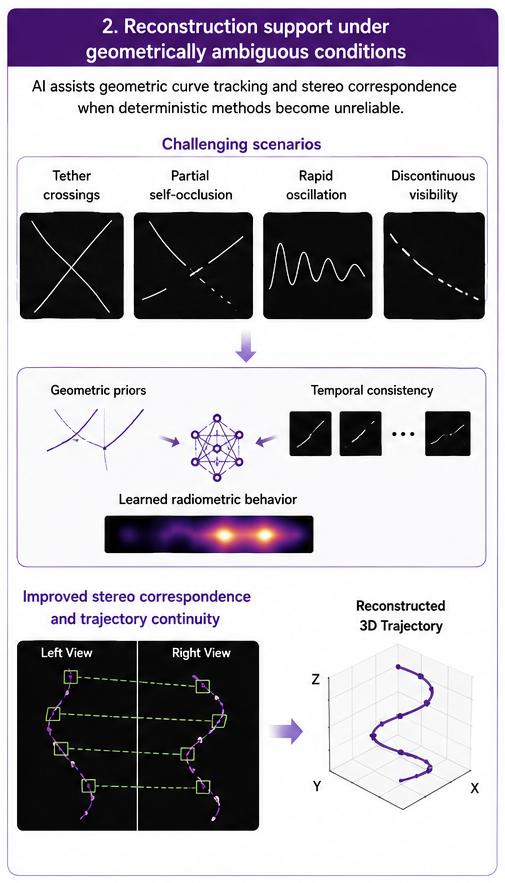
\includegraphics[width=0.5\textwidth]{Images/Figure 4.5.png}
    \caption[Conceptual overview that illustrates reconstruction support under geometrically ambiguous conditions]{Conceptual overview that illustrates reconstruction support under geometrically ambiguous conditions. AI-assisted methods are explored to improve geometric curve tracking and stereo correspondence in scenarios involving tether crossings, partial self-occlusion, rapid oscillatory motion, and discontinuous radiometric visibility. The figure highlights the incorporation of temporal consistency, geometric priors, and learned radiometric behavior to support continuity in reconstruction when deterministic correspondence becomes unreliable.}
    \label{fig:figure4.5}
\end{figure}

\begin{figure}[!ht]
    \centering
    \resizebox{\textwidth}{!}{%
    \begin{tikzpicture}[
        font=\scriptsize,
        node distance = 8mm and 10mm,
        stage/.style    = {rectangle, draw, rounded corners, fill=blue!8,
                           text width=2.8cm, align=center, minimum height=1.3cm},
        decision/.style = {diamond, draw, fill=blue!12, aspect=2.2,
                           text width=2.4cm, align=center, inner sep=1pt},
        today/.style    = {rectangle, draw=gray, dashed, fill=gray!6,
                           text width=4.6cm, align=left, font=\tiny, minimum height=1.3cm},
        proposed/.style = {rectangle, draw=green!45!black, dashed, fill=green!8,
                           text width=4.6cm, align=left, font=\tiny, minimum height=1.5cm},
        dataflow/.style = {rectangle, draw=orange!70!black, fill=orange!8,
                           text width=3.4cm, align=center, font=\tiny, minimum height=1.1cm},
        arr/.style      = {-{Stealth[length=2mm]}, thick},
    ]

    % ---- main search loop (this part already exists, classical) ----
    \node[stage] (mask) {Segmentation mask (Model 1) + skeleton};
    \node[stage, right=of mask] (branch) {Find next branch point along current strand};
    \node[decision, right=of branch] (score) {Score each candidate continuation};
    \node[stage, right=of score] (pick) {Advance to highest-scored candidate};
    \node[stage, right=of pick] (end) {Reached the other end?};
    \node[stage, right=of end, text width=2.4cm] (out) {Output: ordered path (same format as today)};

    \draw[arr] (mask) -- (branch);
    \draw[arr] (branch) -- (score);
    \draw[arr] (score) -- (pick);
    \draw[arr] (pick) -- (end);
    \draw[arr] (end) -- node[above, font=\tiny]{yes} (out);
    \draw[arr] (end.south) to[out=-90,in=-90,looseness=1.4]
        node[below, font=\tiny]{no -- loop} (branch.south);

    \node[above=2mm of mask, font=\bfseries\scriptsize, text width=15cm, align=left]
      {Proposed AI wire path tracker -- one search loop for both untangled and knotted/self-crossing thread configurations};

    % ---- the swappable component ----
    \node[today, below=14mm of score, xshift=-1.4cm] (today-box)
      {\textbf{TODAY (implemented, classical):} fixed hand-tuned weights -- direction continuity $\times$1200 + thickness continuity $\times$600 + centeredness $\times$300 -- parallel-line penalty. Same formula regardless of how tangled the thread is.};
    \node[proposed, below=6mm of today-box] (proposed-box)
      {\textbf{PROPOSED (not implemented):} a lightweight classifier (Random-Forest-style, CPU-only, same philosophy as Model 1) predicts which candidate a human would choose, using the same geometric features plus local image patch. \emph{One trained model is reused at every branch point} -- a clean thread has 0--1 branch points, a knotted thread has many, but each is resolved the same way. This is why wire tracking and knot/crossing resolution are one AI component, not two.};

    \draw[arr, gray] (score.south) -- (today-box.north);
    \draw[arr, green!45!black] (today-box.south) -- (proposed-box.north);

    % ---- training data loop for the proposed scorer ----
    \node[dataflow, below=6mm of proposed-box, xshift=1cm] (dataset)
      {path\_dataset: image + mask + verified path (stereo pairs)};
    \node[dataflow, right=6mm of dataset] (extract)
      {Offline: replay path over skeleton branch points $\rightarrow$ label (features, chosen candidate)};
    \node[dataflow, right=6mm of extract] (train)
      {Train classifier};

    \draw[arr, orange!70!black] (dataset) -- (extract);
    \draw[arr, orange!70!black] (extract) -- (train);
    \draw[arr, orange!70!black] (train.north) |- ($(train.north)+(0,0.6)$) -| (proposed-box.east);

    \end{tikzpicture}}
    \caption[Proposed architecture for the AI-assisted wire path tracker]{Proposed architecture for the AI-assisted wire path tracker. The overall search loop (top row) is unchanged from the classical SmartWireTracker already implemented today: it walks the segmented thread step by step and, at each branch point, scores the candidate continuations to pick the most likely one. The only proposed change is replacing the fixed, hand-tuned scoring formula with a learned scorer trained on the same \texttt{path\_dataset} already being collected (bottom row). Because the same scorer is invoked at every branch point regardless of how many exist, this single component naturally handles both simple, untangled threads (few or no branch points) and heavily tangled or self-crossing configurations (many branch points) -- it is one AI model solving one problem, not two separate systems for ``tracking'' and ``knot solving''.}
    \label{fig:ai-proposed-tracker}
\end{figure}

\newpage
\clearpage

\noindent \textbf{3. Neural rendering and future reconstruction approaches}
\vspace{0.2cm}

The final exploratory direction considers the potential future integration of neural rendering approaches, including Neural Radiance Fields (NeRFs) and related implicit scene representation techniques.
\\\\
These methods may offer future capabilities for multi-view geometric interpretation, radiometric interpolation, and reconstruction of sparse visual structures under limited observation conditions, as illustrated in Figure \ref{fig:figure4.6}.
\\\\
Potential future implementations may additionally incorporate techniques such as \textit{Textual Inversion for tether-specific radiometric adaptation} and \textit{Score Distillation Sampling (SDS) for geometry-consistent neural rendering optimization}
\\\\
However, the direct application of these approaches to orbital tether reconstruction remains constrained by several practical limitations, including a lack of representative datasets, computational complexity, sparse visual texture, and highly dynamic illumination conditions. For this reason, AI integration is currently treated as a future-oriented augmentation layer rather than as the primary operational reconstruction methodology of the LINKU stereo vision system.

\begin{figure}[!ht]
    \centering
    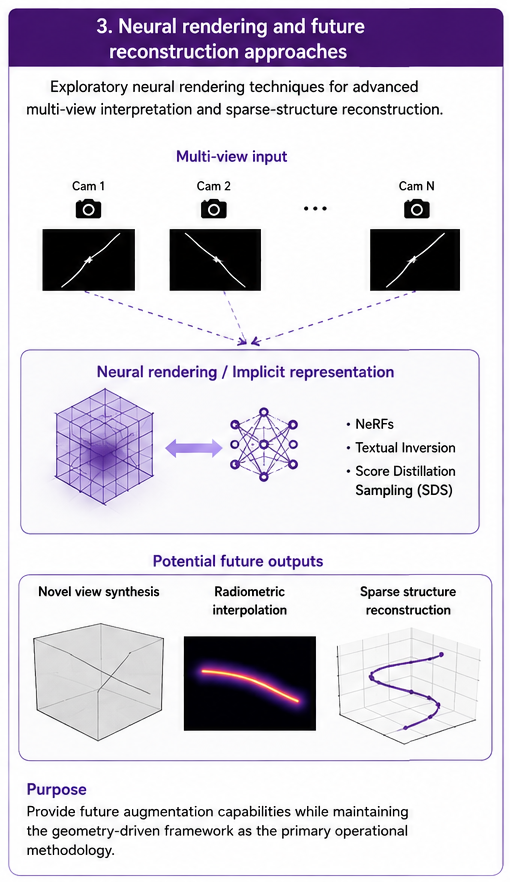
\includegraphics[width=0.5\textwidth]{Images/Figure 4.6.png}
    \caption[Conceptual overview that presents exploratory neural rendering and future reconstruction approaches]{Conceptual overview that presents exploratory neural rendering and future reconstruction approaches based on implicit scene-representation techniques such as Neural Radiance Fields (NeRFs), Textual Inversion, and Score Distillation Sampling (SDS). These methods are investigated for future applications involving multi-view geometric interpretation, radiometric interpolation, sparse-structure reconstruction, and novel-view synthesis under limited observation conditions.}
    \label{fig:figure4.6}
\end{figure}

\newpage
\clearpage

The resulting Phase III framework establishes a preliminary research direction for future system maturation while preserving the geometry-driven reconstruction methodology of Phase II as the principal operational strategy for reconstruction.